\documentclass[margin=2mm]{standalone}

\usepackage{tikz}
\usetikzlibrary{mindmap}

\begin{document}
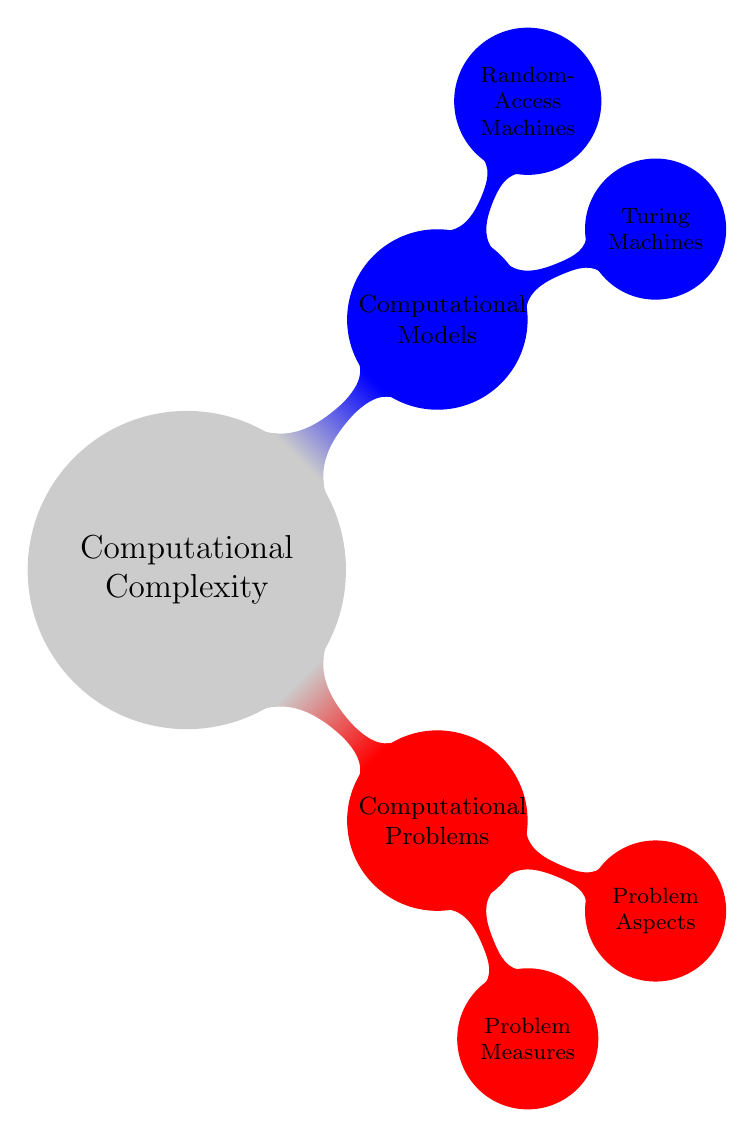
\begin{tikzpicture}[
    mindmap,
    every node/.style=concept,
    concept color=black!20,
    grow cyclic,
    level 1/.append style={level distance=4.5cm,sibling angle=90},
    level 2/.append style={level distance=3cm,sibling angle=45}
    ]
  \node [root concept] {Computational Complexity} % root
    child [concept color=red] { node {Computational Problems}
      child { node {Problem Measures} } 
      child { node {Problem Aspects} }
    }
    child [concept color=blue] { node {Computational Models}
      child { node {Turing Machines} }
      child { node {Random-Access Machines} }
    };
\end{tikzpicture}
\end{document}
